\section{Constrained Application Protocol}

The Constrained Application Protocol (CoAP) is designed to enable web-based services in constrained wireless networks, where traditional web solutions may not be feasible due to hardware and network limitations. 
These constraints include: low-power devices, limited memory and processing capabilities, and energy-efficient, low-bandwidth networks. 
To overcome these challenges, CoAP redesigns web-based communication to suit constrained environments while maintaining compatibility with standard web technologies.

\paragraph*{Features}
CoAP is an embedded web transfer protocol optimized for lightweight, efficient communication. 
It introduces several features tailored for constrained devices:
\begin{itemize}
    \item CoAP URI scheme \texttt{coap://}. 
    \item Asynchronous transaction model which supports non-blocking communication. 
    \item UDP binding with reliability and multicast support. 
    \item RESTful methods. 
    \item URI support. 
\end{itemize}
\begin{figure}[H]
    \centering
    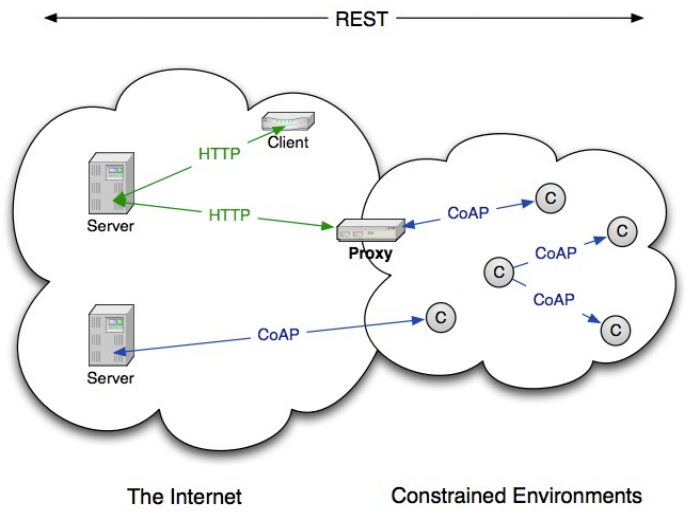
\includegraphics[width=0.5\linewidth]{images/coap.png}
    \caption{CoAP architecture}
\end{figure}
CoAP plays a critical role in IoT ecosystems, enabling lightweight, low-latency communication between resource-constrained devices while maintaining compatibility with traditional web technologies. 
Its UDP-based nature makes it well-suited for low-power wireless networks such as 6LoWPAN, LPWAN, and LoRaWAN, where energy efficiency and bandwidth conservation are key priorities.

\paragraph*{Proxying and caching}
CoAP proxies act as intermediaries between clients and servers, forwarding requests and responses. 
They help with load balancing, security, and NAT traversal, improving network efficiency and scalability.
Caching: CoAP supports caching responses to reduce repeated network requests. 
Clients and proxies can store responses and reuse them if the resource hasn't changed, saving bandwidth and improving speed.

\subsection{Messages}
CoAP primarily relies on UDP for lightweight communication, making it ideal for constrained networks. 
Message exchange occurs between endpoints with a compact 4-byte header, ensuring minimal overhead.
Each message contains a 16-bit Message ID, enabling mechanisms for both reliable and unreliable transmission:
\begin{itemize}
    \item \textit{Confirmable messages}: require acknowledgment (ACK) or may trigger a Reset Message (RST) if lost. 
        A stop-and-wait retransmission strategy with exponential backoff ensures reliability.
    \item \textit{Non-confirmable messages}: sent without requiring acknowledgment, suitable for non-critical or frequent updates.
    \item \textit{Duplicate detection}: both confirmable and non-confirmable messages use Message IDs to identify and discard duplicates.
\end{itemize}
CoAP follows a RESTful architecture, embedding request and response semantics directly into its messages. 
Each message can carry: methods, response code and options. 
\begin{figure}[H]
    \centering
    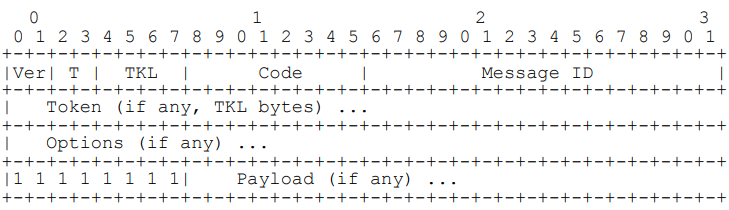
\includegraphics[width=0.5\linewidth]{images/coap1.png}
    \caption{CoAP message}
\end{figure}
The CoAP 4-byte message header consists of several key fields:
\begin{itemize}
    \item \textit{Version} (\texttt{Ver}): CoAP version. 
    \item \textit{Type} (\texttt{T}): defines the message type. 
        The message can be: confirmable (\texttt{CON}), non-confirmable (\texttt{NON}), acknowledgment (\texttt{ACK}), and reset (\texttt{RST}).
    \item \textit{Token length} (\texttt{TKL}): indicates the number of bytes used for the token field.
    \item \textit{Code}: represents either a request method (1 to 10) or a response code (40 to 255).
    \item \textit{Message ID}: a 16-bit identifier for tracking requests and responses.
    \item \textit{Token} (optional): used for request-response matching, especially in asynchronous communication.
\end{itemize}

\subsection{Packet loss}
CoAP employs a stop-and-wait retransmission mechanism to handle packet loss in unreliable networks. 
This approach ensures that lost messages are resent while maintaining low overhead.

When sending a confirmable message, the sender expects an acknowledgment or a reset message. 
If no response is received within a timeout period, the request is retransmitted.
\begin{verbatim}
Rand [ACK_TIMEOUT, ACK_TIMEOUT x ACK_RANDOM_FACTOR] ([2s, 3s])
\end{verbatim}
If no response is received after the initial timeout, and the transmission counter is less than \texttt{MAX\_RETRANSMIT(4)}: the transmission counter is increased, the timeout value is doubled (exponential backoff), and the message is retransmitted.
This process continues until one of the following conditions is met:
\begin{itemize}
    \item An \texttt{ACK} is received, confirming successful delivery.
    \item An \texttt{RST} message is received, indicating rejection.
    \item The transmission counter exceeds \texttt{MAX\_RETRANSMIT} (4 retransmissions).
    \item The total attempt duration surpasses \texttt{MAX\_TRANSMIT\_WAIT} (93 seconds), at which point the transmission is aborted.
\end{itemize}

\subsection{Observation}
In the traditional REST paradigm, data is fetched through explicit pull requests, where the client continuously queries the server for updated information.
In Wireless Sensor Networks, however, data is often periodic or triggered by specific events.

CoAP introduces the concept of Observation to address this issue. 
Observation allows clients to subscribe to resources and receive updates automatically whenever the resource's state changes, without having to repeatedly poll the server. 
This is more efficient, as it reduces unnecessary requests and bandwidth consumption.

CoAP clients use the \texttt{observe} option in their requests to subscribe to a resource.
When the resource state changes, the server sends an update to the client.
The client is notified asynchronously, receiving updates as they occur without needing to send explicit requests.

\subsection{Block transfer}
In networks using IPv6, large payloads are often fragmented at the lower layers, which can be inefficient. 
This can create overhead when transferring large data sets.
CoAP uses Block Transfer at the application layer to handle large messages by splitting them into smaller blocks, avoiding fragmentation at lower layers.
Block Transfer adds an option to CoAP messages, including:
\begin{itemize}
    \item \texttt{nr}: incremental block number within the original data.
    \item \texttt{m}: a flag indicating if more blocks are expected.
    \item \texttt{sz}: block size, which determines the chunk size for each transfer.
\end{itemize}

\subsection{Discovery}
CoAP supports resource discovery, allowing clients to discover and interact with available resources on CoAP servers.
The goal is to enable clients to discover the links hosted by a CoAP (or HTTP) server, including details like the URL, resource type, content type, and supported operations.
The server returns resource details in a link-header format, which includes:
\begin{itemize}
    \item \textit{URL}: the resource location.
    \item \textit{Relation}: describes the relationship between resources.
    \item \textit{Type}: specifies the resource type.
    \item \textit{Content-type}: indicates the format of the resource.
    \item \textit{Interface}: describes the access protocol.
\end{itemize}